

\chapter{序論}

\section{本研究の背景}
日本において,都市部や観光地での交通渋滞は日常的に見られる光景である.特に人気の高い施設の周辺道路では,空きのある駐車場を求める車両によって大きな渋滞を引き起こすケースがある.

\begin{figure}[htb]
	\centering
	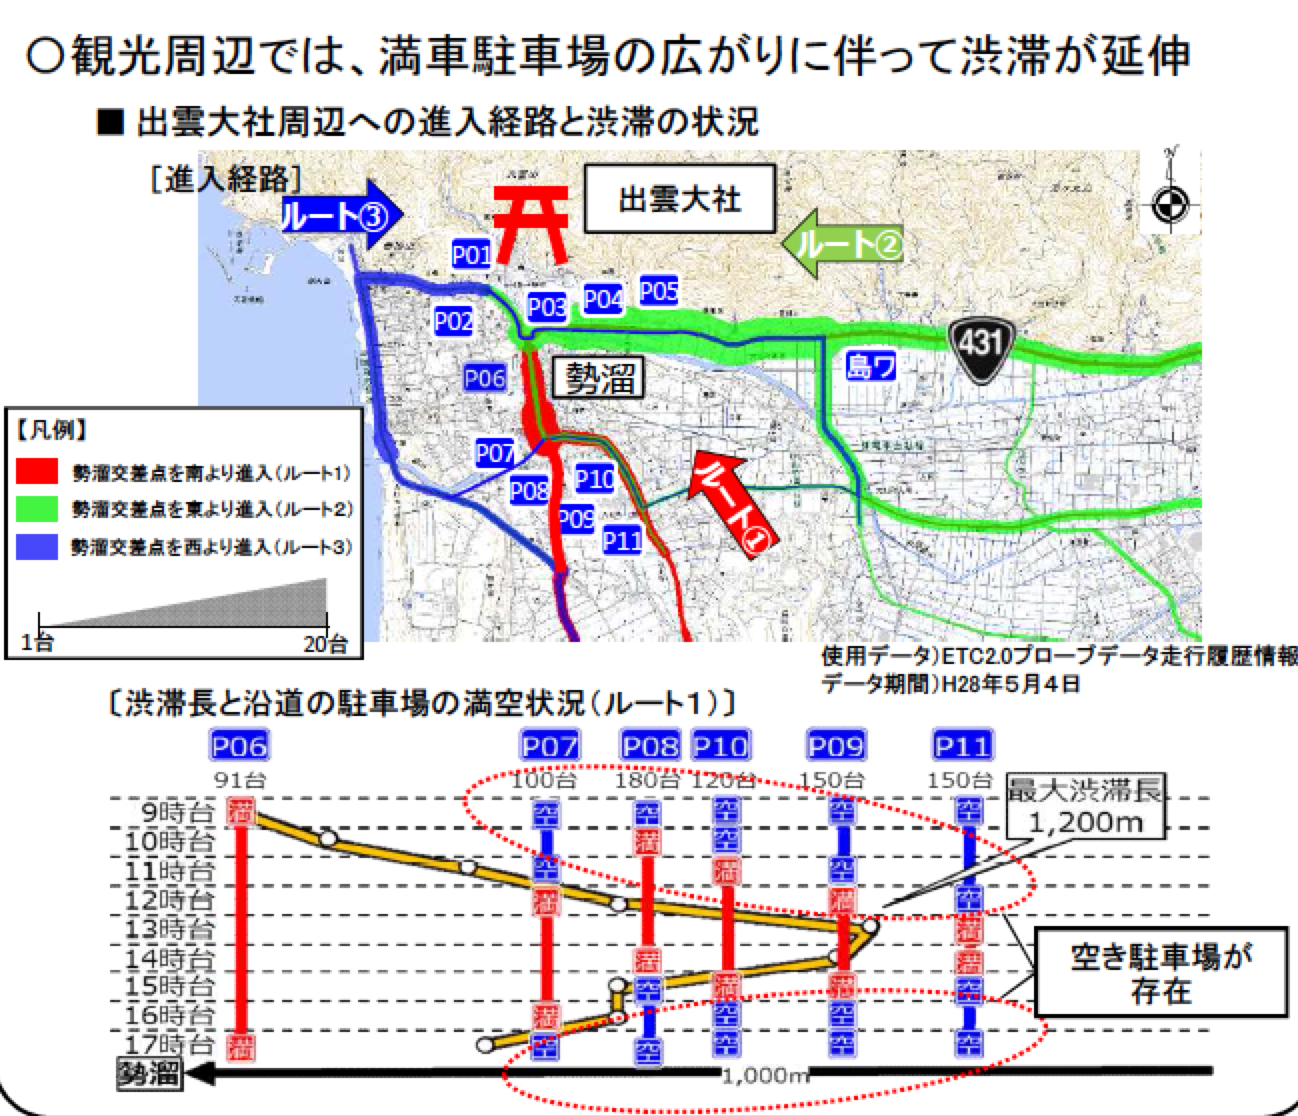
\includegraphics[width=12cm]{fig/kokudo-fig.png}
	\caption{駐車場の空き待ち行列の発生に伴う周辺道路の渋滞の増加 \protect \footnotemark}
	\label{kokudo-fig}
\end{figure}
\footnotetext{国土交通省の配布資料より引用\cite{Kokudo}}


国土交通省の調査\cite{Kokudo}によると,一部の人気観光地において駐車場待ちによる渋滞が多発している一方で,近傍には空きのある駐車場が存在するケースが報告されている.図\ref{kokudo-fig}に駐車場の空き待ち行列の発生に伴う周辺道路の渋滞の発生をグラフに示す.

これらのような環境では,空きのある駐車場の可視化や利用者の誘導を行うシステムが求められていたが,近年では事前予約システムや空き待ち予約システムなどの試験的な導入が決まっている.その一例として,国土交通省は図\ref{kokudo-fig-2}のように周辺駐車場への誘導から交通の分散と周遊観光の拡大を目指すシステムを提案している.


\begin{figure}
	\centering
	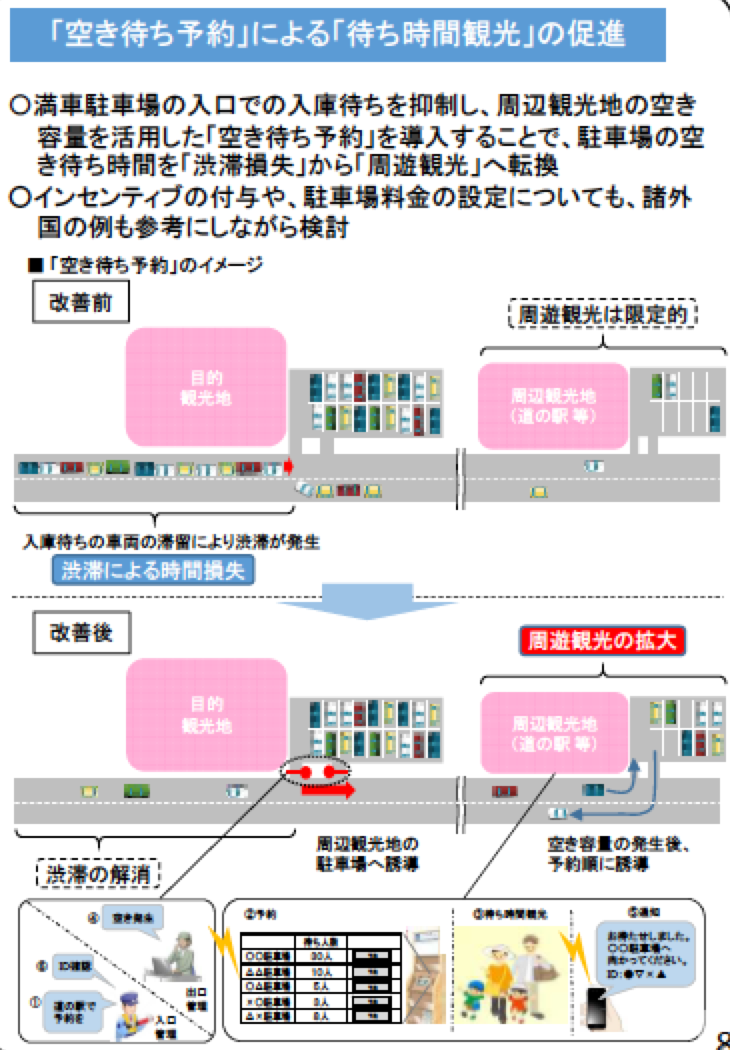
\includegraphics[width=10cm]{fig/kokudo-fig-2.png}
	\caption{導入が進められている駐車場空き待ち予約システム \protect \footnotemark}
	\label{kokudo-fig-2}
\end{figure}
\footnotetext{国土交通省"観光地における渋滞対策"より引用\cite{Kokudo}}
しかし,これらのプラットフォームを効果的に運用するためには,各駐車場のシステムの統合的な管理$\cdot$運用が求められる.管理$\cdot$運用コストの高さから常設機器の設置が困難なため二の足を踏む駐車施設も多い.駐車場は運営者が個人$\cdot$民間$\cdot$行政とまたがるため,それぞれの駐車場に統一した設備を設置するのは大きな障壁になる.




\section{本研究の目的}
既存の駐車場満空システムでは,運営主体による積極的な投資$\cdot$運営$\cdot$管理が必要であった.すなわち,駐車場の効率化の主体はあくまで運営者にあったとも言える.


本研究では車両の位置情報と携帯電話回線網を用いて,駐車場全体のネットワークモデルを自律的に生成する手法を提案する.これにより昨今多方面で提案されていた車両のセンサーを用いる駐車場効率化手法を,運営主体の枠組みを超えて統合的に行うことが可能になる.


\section{本論文の構成}

本論文の構成を以下に示す. 
第\ref{related}章では本研究に関連する技術や先行研究を述べる.第\ref{proposal}章では本提案手法の目的と仮説,具体的なアプローチに関して述べる.第\ref{implementation}章には評価実験を行うシミュレータの実装について記述する.第\ref{evaluation}章では評価実験の概要と結果,考察について述べる.第\ref{conclusion}章では本研究のまとめを記述する.

